\documentclass[../mainfile.tex]{subfiles}


\begin{document}
\section{Quadratic variation}
\subsection{Quadratic variation of continuous martingales}
\subsubsection{Warm-up via embedded random walks}
Let us revisit what we did in the proof of Donsker's theorem: We considered a Brownian motion started from $0$ and we defined for all $\epsilon>0$ iteratively the stopping times 
\begin{align*}
T_0^\epsilon:=0, \ T_{n+1}^\epsilon = \inf \{ t >T_n^\epsilon : |B_t-B_{T_n^\epsilon}| = \epsilon\}.
\end{align*}
The walk given by $Z_n:= B_{T_n^\epsilon}$ is then a fair random walk that moves up or down by $\pm \epsilon$ at each step. If we define $Z^p:= (Z_n^p)_{n \geq 0}$ to be the walk corresponding to the specialized $\epsilon_p= 2^{-p}$, we then note that we can recover the walk $Z^p$ from the knowledge of $Z^{p+1}$, we say that the sequence of walks $Z^p$  is nested.
\\\\
To summarize our ideas above: Given a Brownian motion, then the Brownian motion defines a nested family of walks $Z^p$ (for $p \geq 0$) of random walks on finer and finer meshes. 
\\\\
One feature that we established during the course of the proof of Donsker's theorem is that the knowledge of all the nested walks $Z^p$ allows to recover $B$. Indeed, we have seen that for each given $t \geq 0$, we have that 
\begin{align*}
T_{[ t \epsilon^{-2}]}^\epsilon \overset{\mathbb{P}}\longrightarrow t, \text{ as } \epsilon \to 0.
\end{align*}
In particular, by Donsker's theorem, this implies that 
\begin{align*}
B_t =\lim_{p \to \infty}^\mathbb{P} Z^p_{[t \epsilon_p^{-2}]} = \lim_{p \to \infty}^\mathbb{P} Z^p_{[t4^p]},
\end{align*}
which shows that one can recover all the trajectory and time-parametrization of $B$ from the knowledge of the nested family of random walks $Z^p$. 
\newpage
We will now apply the same idea to continuous martingales. Suppose that $(M_t)_{t \geq 0}$  is a continuous martingale with respect to some filtration $( \mathcal{F}_t)_{t \geq 0}$ with $M_0=0$ almost surely, let us also assume (for reasons of simplicity) that $\limsup_{t \to \infty} M_t = \infty$. 
\\\\
We can then define in exactly the same fashion as we defined $T_n^\epsilon$ for $B$ the sequence of stopping times $S_0^\epsilon =0$ and for all $n \geq 1$:
\begin{align*}
S_n^\epsilon:= \inf \{ t > S_{n-1}^\epsilon : |M_t-M_{S_{n-1}^\epsilon}|= \epsilon\}. 
\end{align*}
The condition about the limsup of $M$ ensures that all these stopping times are finite, and the continuity of $M$ ensures also that for each $\epsilon >0$ we have $S_n^\epsilon \to \infty$ as $n \to \infty$ (as otherwise, $\limsup_{n \to \infty} M_{S_n^\epsilon} = \infty$). 
\\
\\
Let us look at the case $n=1$, then the stopped martingale $M^{S_1^\epsilon}$ is bounded (it's bounded by $\epsilon$) and thus in particular uniformly integrable, by the optional stopping theorem we obtain 
\begin{align*}
\mathbb{E}(M_{S_1^\epsilon}) = \mathbb{E}(M_0)=0 \implies \mathbb{P}(M_{S_1^\epsilon}= \epsilon)= \mathbb{P}( M_{S_1^\epsilon}= - \epsilon)= \frac{1}{2}.
\end{align*}
But also by the optional stopping time (more elaborate version) we get that 
\begin{align*}
\mathbb{E}(M_{S_{n+1}^\epsilon} \mid \mathcal{F}_{S_n^\epsilon}) = M_{S_n^\epsilon} \iff \mathbb{E}(M_{S_{n+1}^\epsilon}-M_{S_n^\epsilon} \mid \mathcal{F}_{S_n^\epsilon}) =0 
\\
\implies \mathbb{P}(M_{S_{n+1}^\epsilon}-M_{S_n^\epsilon} = \pm \epsilon \mid \mathcal{F}_{S_n^\epsilon}) = \frac{1}{2}
\end{align*}
This shows that the walk $Y_n:= M_{S_n^\epsilon}$ is a fair random walk that moves up or down $\pm \epsilon$ at each step. So, if we define $Y^p$ to be the walk corresponding to $\epsilon_p = 2^{-p}$, we get that the walks $Y^p$ for $p \geq 1$ are nested exactly as the walks $Z^p$ were. In other words,  the nested sequence of random walks $(Y_n^p, \geq 0 )_{p \geq 1}$ and $(Z_n^p, n \geq 0 )_{p \geq 1}$ have the same law. 
\\\\
In particular, this shows that starting from the trajectory of a continuous martingale $M$, one can first define the nested family $Y^p$, then define $Z^p$ to be equal to $Y^p$ and then one can construct a Brownian motion $B$ from this nested family $Z^p$ using the procedure we have described on the previous page (using Donsker's invariance theorem). In other words, starting from a continuous martingale $M$, one can define a Brownian motion $B$ which is some deterministic function of $M$. 
\newpage
\textbf{Recap:} \textit{Starting with a continuous martingale $M$, one can define a Brownian motion $B$ which is some deterministic function of $M$.}
\\\\
Lets make this more concrete: for each time $t$, we can define $N_\epsilon(t)$ to be the largest integer $n \in \mathbb{N}$ such that $S_n^\epsilon \leq t$. In other words, $N_\epsilon(t)$ is the number of $\epsilon$-steps performed by $M$ up to time $t$, in particular we have \begin{align*}
|M_t-Y_{N_\epsilon(t)}| \leq \epsilon, \text{ (where } Y_n=M_{S_n^\epsilon})
\end{align*}
We therefore conclude that (see picture in proof of Donsker's theorem), as $\epsilon \to 0$, $\epsilon^2 N_\epsilon(t)$ converges in probability to the time $A_t$ such that $B_{A_t}=M_t$. It suggests therefore that if one defines 
\begin{align*}
A_t:= \lim_{ \epsilon \to 0}^\mathbb{P} \epsilon^2 N_\epsilon(t),
\end{align*}
then it will be possible to define a continuous modification of the process $(A_t)_{t \geq 0}$ such that for all $t \geq 0$ we have \begin{align*}
M_t=B_{A_t}. \tag{*}
\end{align*}
This continuous process $(A_t)_{t \geq 0}$ is what we will call the \textbf{quadratic variation} of the martingale $M$. One often refers to (*), as the fact that $M$ is a time-changed Brownian motion. 
\begin{figure}[hbtp]
\centering
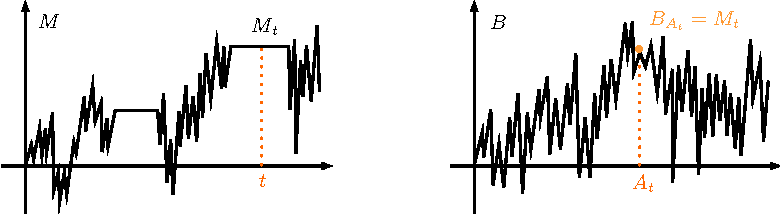
\includegraphics[scale=1]{quadvarproc.pdf}
\caption{Notice that as $\epsilon \to 0$, according to the definition of $N_\epsilon(t)$ we count "$0$"-steps. The picture then displays the time change of a Brownian motion.}
\end{figure}
\\
In the next section, we will in fact construct this quadratic variation by other means, but then check that indeed it corresponds to the process $A_t= \lim_{ \epsilon \to 0} \epsilon^2 N_\epsilon(t)$. 
\newpage
\subsubsection{Quadratic variation of bounded martingales}
\textbf{Idea:} We know that $B_t^2 -t$ is a continuous martingale, this suggests that the time-changed process 
\begin{align*}
(B_{A_t}^2-A_t)_{t \geq 0}=(M_t^2-A_t)_{t \geq 0}
\end{align*}
will be a (sort of) martingale (or rather what we will call a local martingale). We will in fact show that this feature, that $A=(A_t)_{t \geq 0}$ is a continuous non-decreasing process such that $((M_t)^2-A_t)_{t \geq 0}$ is a local martingale does characterize $A$ uniquely and provides a neat way to construct it. 
\\\\
Let us now suppose that $(M_t)_{t \geq 0}$ is a continuous martingale that is started from $0$ such that: 
\begin{itemize}
\item $|M|$ is almost surely bounded by some deterministic constant $C$ (i.e., almost surely, for all $t \geq 0$, $|M_t| \leq C)$. 
\item For some deterministic integer $K$, $M$ is almost surely constant on $[K, \infty)$ (i.e., almost surely,  for all $t \geq K$, $M_t=M_K)$. 
\end{itemize}
These two conditions look at first pretty restrictive, but we shall see that it will be easy to deduce the general results for continuous martingales from the results that we derive with these two restrictions. In other words,  everything happens here, all the core arguments of the construction of the quadratic variation of continuous martingales. We also already mention here that the quadratic variation will be at the core of our definitions of stochastic integrals. 
\\\\
The key result (under the \textit{'restrictions'} above) of this section will be the following:
\begin{prop} There exists a unique continuous non-decreasing process $(A_t)_{t \geq 0}$ with $A_0=0$ ($A_t$ is $\mathcal{F}_t$-measurable and in $L^2)$ such that $(M_t^2-A_t)_{t \geq 0}$ is an $L^2$-martingale. 
\end{prop}
\begin{defn} This unique process $(A_t)_{t \geq 0}$ will be called the quadratic variation of the martingale $M$.
\end{defn}
\newpage
The next definitions are crucial:
\begin{defn} When $t \geq 0$, we say that $\Delta_n$ is a nested sequence of subdivisions of $[0,t]$ such that $| \Delta_n| \to 0$ as $n \to \infty$ if:
\begin{itemize}
\item Each $\Delta_n$ consists of a finite family $(t_i^n)_{i \leq m_n}$ such that $0=t_0^n < t_1^n < \dots < t_{m_n}^n =t$ (i.e. it is a subdivision of the interval $[0,t])$.
\item The mesh-size $|\Delta_n|:= \max_{0 \leq i \leq m_n} (t_{i+1}^n-t_i^n)$ tends to $0$ as $n \to \infty$. 
\item The sequence ($\Delta_n)_{n \geq 0}$ of subdivisions is nested, meaning that for each $n \leq n'$ and each $i \leq m_n$, there exists $i' \leq m_{n'}$ such that $t_i^n=t_{i'}^{n'}$.
\end{itemize}
\end{defn}
\begin{defn} When $\Delta_n$ is a subdivision of $[0,t]$, we then define 
\begin{align*}
V_{\Delta_n}:= \sum_{i=0}^{m_n-1} (M_{t_{i+1}^n}-M_{t_i^n})^2 
\end{align*}
to be the sum of the squares of the increments of $M$ along the subdivision $\Delta_n$. We will refer to $V_{\Delta_n}$ as the \textbf{discrete quadratic variation} of $M$ along the subdivision $\Delta_n$. 
\end{defn}
\begin{prop} If $\Delta_n$ is a nested sequence of subdivisions of $[0,t]$ with $|\Delta_n| \to 0$ (mesh sizes tends to $0$), then the sequence $V_{\Delta_n}$ converges in $L^2$ to $A_t$. 
\end{prop}
We will prove both propositions at once: 
\begin{proof}
\textbf{Uniqueness:} Let us suppose that there were two such process $A$ and $A'$. Note that $A$ and $A'$ are then necessarily in $L^2$, since they are the difference between two processes that are in $L^2$ (namely the bounded process $(M_t^2)_{t \geq 0}$ and the $L^2$ martingales given by $M^2-A$ respectively $M^2-A'$). Let us define $(A_t'':= A_t-A_t')_{t \geq 0}$ which is an $L^2$ martingale.
\\\\
Let us consider a nested sequence $\Delta_n$ of subdivisions on $[0,K]$ with $|\Delta_n| \to 0$. 
\begin{align*}
\mathbb{E}((A_K'')^2) &= \sum_{i=0}^{m_n-1} \mathbb{E} ((A_{t_{i+1}^n}''-A_{t_i^n}'')^2) \\ & \leq \mathbb{E}( \max_{i \leq m_n-1} |A_{t_{i+1}^n}''-A_{t_i^n}''| \times \sum_{i=0}^{m_n-1} |A_{t_{i+1}^n}''-A_{t_i^n}''|) \\
& \overset{\Delta}\leq \mathbb{E}( \max_{i \leq m_n-1} |A_{t_{i+1}^n}''-A_{t_i^n}''| \times \sum_{i=0}^{m_n-1} ( | A_{t_{i+1}^n}-A_{t_i^n}| + |A_{t_{i+1}^n}'-A_{t_i^n}'|)) \\
& \leq \mathbb{E}( \max_{i \leq m_n-1} |A_{t_{i+1}^n}''-A_{t_i^n}''| \times (A_K+A_K')).
\end{align*}
Where in the last inequality we used the fact that $A$ and $A'$ are non-decreasing.
\newpage
But by the continuity of $A$ and $A'$ we have that almost surely
\begin{align*}
\max_{i \leq m_n-1} |A_{t_{i+1}^n}''-A_{t_i^n}''| \to 0 \text{ as } n \to \infty.
\end{align*}
On the other hand, 
\begin{align*}
\max_{i \leq m_n-1} |A_{t_{i+1}^n}''-A_{t_i^n}''| \times (A_K+A_K') \\ \overset{\Delta}\leq \max_{i \leq m_n-1}( | A_{t_{i+1}^n}-A_{t_i^n}| + |A_{t_{i+1}^n}'-A_{t_i^n}'|) \times (A_K+A_K') \leq (A_K + A_K')^2 
\end{align*}
where we used again that $A$ and $A'$ are non-decreasing, since we also know that $A_t+A_t'$ is in $L^2$, we can apply dominated convergence for $n \to \infty$ to obtain that 
\begin{align*}
\mathbb{E}((A_K'')^2) =0. 
\end{align*}
Since $(A_t'')_{t \geq 0}$ is an $L^2$-martingale (as the difference of $L^2$ martingales), we can apply Doob's $L^2$ inequality to establish 
\begin{align*}
\mathbb{E}( \sup_{t \leq K} (A_t'')^2) \leq 4 \mathbb{E}((A_K'')^2) =0
\end{align*}
from which we conclude that almost surely $A_t''=0$ for all $t \leq K$, and thus $A=A'$ as processes. 
\\\\
\textbf{Existence:} \textit{Only idea of the proof.}\\
\\
Instead of trying to approximate the process $(A_t)_{t \geq 0}$, we first try to find the right approximation of the martingale $2X_t:= M_t^2-A_t$. We take a nested sequence $\Delta_n$ of subdivisions of $[0,K]$ such that the mesh-size $|\Delta_n|$ tends to $0$ as $n \to \infty$ and then for each $n \in \mathbb{N}$ we define
\begin{align*}
X_t^n := \sum_{i=0}^{m_n-1} M_{t_i^n} (M_{t \wedge t_{i+1}^n}- M_{t \wedge t_i^n}), 
\end{align*}
we notice that this is a bounded continuous martingale such that on each interval $[t_i^n, t_{i+1}^n]$, the increments of this martingale are exactly $M_{t_i^n}$ times the increments of $M$. In other words, for all $t \in [t_i^n, t_{i+1}^n]$ we have
\begin{align*}
X_t^n-X_{t_i^n}^n = M_{t_i^n} \times (M_t-M_{t_i^n}). 
\end{align*}
\newpage
The idea is that $2X_t^n$ is a martingale that will approximate $M_t^2-A_t$ well. Indeed we have \begin{align*}
V_{\Delta_n} = \sum_{i=0}^{m_n-1} ( M_{t_{i+1}^n}-M_{t_i^n})^2 \text{ and } 2X_K^n = \sum_{i=0}^{m_n-1} 2M_{t_i^n}(M_{t_{i+1}^n}-M_{t_i^n})
\end{align*}
from which we can conclude that
\begin{align*}
V_{\Delta_n} + 2X_K^n &= \sum_{i=0}^{m_n-1} (M_{t_{i+1}^n}-M_{t_i^n}+2M_{t_i^n})(M_{t_{i+1}^n}-M_{t_i^n}) \\
&= \sum_{i=0}^{m_n-1} (M_{t_{i+1}^n}^2-M_{t_i^n}^2) = M_K^2-M_0^2=M_K^2 
\end{align*}
So, if we can show that $X_K^n$ converges in $L^2$ to some $X_K$ as $n \to \infty$, we conclude that $V_{\Delta_n}$ does converge in $L^2$ to $M_K^2-2X_K$.
\\\\
We now briefly outline the rest of the proof:
\begin{itemize}
\item \textbf{Step 1:} \textbf{Lemma:} $X_K^n$ converges in $L^2$ to some random variable $X_K$ as $n \to \infty$. Establishing this Lemma is quite technical and will be skipped. 
\item \textbf{Step 2:} There exists a sequence $n_k \to \infty$, such that almost surely $X^{n_k}$ converges uniformly on $[0,K]$ to a continuous function $(X_t)_{t \leq K}$ ($X_t=X_K$ for $t \geq K)$ and we check that $(X_t)_{t \geq 0}$ is an $L^2$-martingale. 
\item \textbf{Step 3:} Finally we check that $A_t:= M_t^2-2X_t$ is a continuous, adapted $L^2$ process which is non-decreasing. (The non-decreasing part is again a bit technical).
\end{itemize}
\end{proof}
\begin{rem} Let us comment on the martingale $(M_t^2-A_t)_{t \geq 0}$ in our construction. What we have seen is that when $M_0=0$ almost surely, then for all $K$, if one chooses a nested sequence $(\Delta_n)_{n \geq 0}$ of subdivisions of $[0,K]$ with $|\Delta_n| \to 0$, then for all $t \leq K$, $M_t^2-A_t$ is "twice" the limit in $L^2$ of 
\begin{align*}
\sum_{i=0}^{m_n-1} M_{t_i^n} (M_{t \wedge t_{i+1}^n}- M_{t \wedge t_i^n}).
\end{align*}
This limiting martingale is what we will call the stochastic integral $\int_0^t M_sdM_s$ when we will define stochastic integrals. So we can write
\begin{align*}
(M_t)^2 = 2 \int_0^t M_sdM_s + A_t. 
\end{align*}
\end{rem}
\newpage
\subsubsection{Quadratic variation of general $L^2$ martingales}
In the previous section, we have constructed and characterized the quadratic variation of a martingale $(M_t)_{t \geq 0}$ under the assumption that $|M|$ was bounded by some deterministic constant $C$ and that it was almost surely constant after some deterministic time $K$. As we will explain now, neither assumption is actually needed to show the existence and uniqueness of the quadratic variation of a martingale. We remark that the condition that $M$ is in $L^2$ is actually needed in order to ensure that the process $(M_t^2-A_t)_{t \geq 0}$ is in $L^1$, and can therefore be a martingale. 

\begin{thm}[Quadratic variation for $L^2$ martingales] There exists a unique adapted continuous non-decreasing process $(A_t)_{t \geq 0}$ with $A_0=0$ such that $(M_t^2-A_t)_{t \geq 0}$ is a martingale. Furthermore, for all $ t \geq 0$, and for all choice of nested sequences $\Delta_n$ of subdivisions of $[0,t]$ with $|\Delta_n| \to 0 $, $V_{\Delta_n}$ converges in probability to $A_t$ as $n \to \infty$. 
\end{thm}
\subsubsection{Quadratic variation of local martingales}
\textbf{Motivation:} Assume we are given a Brownian motion $(B_t)_{t \geq 0}$ started from $0$ and a random variable $Z$ that is independent of $B$. We then can define 
\begin{align*}
M_t:= Z + B_t,
\end{align*}
i.e. a \textit{"Brownian motion started from a random point $Z$"}. We would like to say that $M$ is like a martingale and that its quadratic variation at time $t$ is given by $t$. However, if $Z \notin L^1$, we cannot say this. 
\begin{defn} A continuous adapted process $(M_t)_{t \geq 0}$ is said to be a local martingale started from $0$ (in some filtered probability space) if: 
\begin{itemize}
\item $M_0=0$ almost surely.
\item There exists a sequence of non-decreasing stopping times such that $T_n \to \infty$ almost surely and $(M_t^{T_n})_{t \geq 0}$ is a continuous martingale started from $0$. 
\end{itemize}
\end{defn}
Equivalent to this is the following definition:
\begin{defn} A continuous adapted process $(M_t)_{t \geq 0}$ is said to be a local martingale if $M_0$ is $\mathcal{F}_0$-measurable and there exists a sequence of non-decreasing stopping times such that $T_n \to \infty$ almost surely and $(M_t^{T_n}-M_0)_{t \geq 0}$ is a continuous martingale. 
\end{defn}
\newpage
\begin{rem} According to our definition, local martingales are always continuous. 
\end{rem}
\begin{lem} $(M_t)_{t \geq 0}$ is a local martingale started from $0$ if and only if:
\begin{itemize}
\item $M_0=0$ almost surely.
\item $M$ is almost surely continuous.
\item If we define $\sigma_n = \inf \{ t > 0 : |M_t|=n \}$ for all $n \in \mathbb{N}$, then $M^{\sigma_n}$ is a martingale. 
\end{itemize}
\end{lem}
\begin{proof}
Easy exercise (from exercise sheets). 
\end{proof}
\begin{lem} If a local martingale started from $0$ has finite variation (meaning that it can be written as the difference between two adapted continuous non-decreasing processes), then it is almost surely equal to $0$ for all times. 
\end{lem}
\begin{proof}
Very similar to the uniqueness proof we have shown in the previous Proposition. 
\end{proof}
It's quite evident from the definition of local martingales, that every continuous martingale (started from $0$) is a local martingale (because we can take any sequence of increasing stopping times that diverges to $\infty$ and already know that the stopped martingale is a continuous martingale). We ask us when is a local martingale a (true) martingale?
\begin{lem} Every \textit{bounded} local martingale is a continuous martingale.  
\end{lem}
\begin{proof}
Let $(M_t)_{t \geq 0}$ be a local martingale that is bounded by some constant $C$, i.e. we have $|M_t| \leq C$ for all $t \geq 0$. Let $(\tau_n)_{n \in \mathbb{N}}$ be a localizing sequence for $M$, i.e. it is a non-decreasing sequence of stopping times such that $(M_t^{\tau_n})_{t \geq 0}$ is a martingale for any $n \in \mathbb{N}$ and $\tau_n \nearrow \infty$ almost surely. Fix $s \leq t$,  by the martingale property we have 
\begin{align*}
\mathbb{E}(M_{t \wedge \tau_n} \mid \mathcal{F}_s) = M_{s \wedge \tau_n}.
\end{align*}
By dominated convergence theorem, which we can apply by the uniform boundedness of $M$, we get that (since $\tau_n \nearrow \infty$) 
\begin{align*}
\mathbb{E}(M_t \mid \mathcal{F}_s) = \lim_{n \to \infty} \mathbb{E}(M_{t \wedge \tau_n} \mid \mathcal{F}_s) = \lim_{n \to \infty} M_{s \wedge \tau_n} = M_s 
\end{align*}
which shows that indeed $M$ is a (true) martingale. 
\end{proof}
\begin{rem} The proof of the Lemma above suggests that it is sufficient to check that $(M_t^{\tau_n}) \to M_t$ in $L^1$ in order to conclude that a local martingale is a martingale. Notice that the previous limit is indeed taken with respect to $n$ as $n \to \infty$. 
\end{rem}
\newpage
We can now state the main results about the quadratic variation of local martingales.
\begin{thm}[Quadratic variation of local martingales] If $(M_t)_{t \geq 0}$ is a local martingale started from $0$, then there exists a unique adapted continuous non-decreasing process $(A_t)_{t \geq 0}$ with $A_0=0$ almost surely and such that $(M_t^2-A_t)_{t \geq 0}$ is a local martingale. Furthermore, for all $t \geq 0$ and for all choice of nested sequences $\Delta_n$ of subdivisions of $[0,t]$ with $|\Delta_n| \to 0$ 
\begin{align*}
V_{\Delta_n} = \sum_{i=0}^{m_n-1} (M_{t_{i+1}^n}-M_{t_i^n})^2 \overset{\mathbb{P}}\longrightarrow A_t, \text{ as } n \to \infty. 
\end{align*}
\end{thm}
\subsubsection{Crossvariation between local martingales}
It is convenient to denote the quadratic variation of a local martingale $M$ by $( \langle M \rangle_t)_{t \geq 0}$. It is natural and useful to also define the \textit{cross-variation} between two local martingales (defined w.r.t. the same filtration). 
\begin{defn}[Crossvariation] If $M$ and $N$ are local martingales, then one defines the process $( \langle M, N \rangle_t )_{t \geq 0}$ and calls this the cross-variation between $M$ and $N$, by 
\begin{align*}
\langle M, N \rangle_t := \frac{1}{4} ( \langle M + N \rangle_t - \langle M-N \rangle_t). 
\end{align*}
\end{defn}
By our previous results we can say that:
\begin{itemize}
\item For all $t \geq 0$, and for all nested sequence $\Delta_n$ of subdivisions of $[0,t]$ with $|\Delta_n| \to 0$, 
\begin{align*}
\sum_{i=0}^{m_n-1} (M_{t_{i+1}^n}-M_{t_i^n})(N_{t_{i+1}^n}-N_{t_i^n}) \overset{\mathbb{P}}\to \langle M, N \rangle_t \text{ as } n \to \infty. 
\end{align*}
\begin{itemize}
\item If $M$ and $N$ are in $L^2$, then this convergence takes place in $L^2$.
\end{itemize}
\item Furthermore, $\langle M, N \rangle$ is the only continuous process with bounded variation (i.e., that can be written as the difference of two non-decreasing adapted processes) such that $MN- \langle M,N \rangle$ is a local martingale. 
\end{itemize}
\begin{rem} With this notation, we set $\langle M \rangle_t = \langle M, M \rangle_t.$
\end{rem}
\end{document}